\chapter{概率基础}\label{chap:probability_space}

\begin{introduction}[考试重点]
    \item 古典概型与几何概型
    \item 条件概率与独立
\end{introduction}

\section{概率空间}

\subsection{随机事件}

\begin{definition}[样本空间]
    \textbf{随机试验}(trial)可能出现的\underline{基本}结果称为\textbf{样本点}(sample point),记为$\omega$;样本点的全体构成\textbf{样本空间}(sample space),记为$\Omega=\{ \omega \}$。
\end{definition}

\begin{definition}[离散样本空间]
    若样本空间中包含至多可数个样本点,则称其为\textbf{离散样本空间}。
\end{definition}

\begin{definition}[事件的古典定义]
    若干样本点$\omega$构成的集合(即$\Omega$的某个子集)称为(随机)\textbf{事件}(event)。
\end{definition}

随机现象被抽象为集合。事件间的包含、等价、互不相容关系,对应成集合间的包含、相等、不相交;逻辑运算(且、或、非等)对应成集合论运算(交、并、补等)。

\begin{example}
    设$A$、$B$、$C$是某个随机现象的三个事件, 则
    \begin{itemize}
        \item 事件“$A$与$B$发生,$C$不发生”可表示为:$AB\overline{C}$.
        \item 事件“$A$、$B$、$C$中至少有一个发生”可表示为:$A \cup B \cup C$.
        \item 事件“$A$、$B$、$C$中至少有两个发生”可表示为:$AB \cup AC \cup BC$.
        \item 事件“$A$、$B$、$C$中恰好有两个发生”可表示为:$AB\overline{C} \cup A\overline{B}C \cup \overline{A}BC$.
        \item 事件“$A$、$B$、$C$同时发生”可表示为:$ABC$.
        \item 事件“$A$、$B$、$C$都不发生”可表示为:$\overline{A} \cap \overline{B} \cap \overline{C}$.
        \item 事件“$A$、$B$、$C$不全发生”可表示为:$\overline{A} \cup \overline{B} \cup \overline{C}$.
    \end{itemize}
\end{example}

\begin{property}
    集合的运算性质:
    \begin{itemize}
        \item 交换律
              \begin{equation}\label{eq:commutativity_set}
                  A \cup B = B \cup A, \quad AB = BA
              \end{equation}
        \item 结合律
              \begin{equation}
                  (A \cup B) \cup C = A \cup(B \cup C), \quad (AB)C = A(BC)\label{eq:associative_law_set}
              \end{equation}
        \item 分配律
              \begin{gather}
                  (A \cup B) \cup C = A \cup(B \cup C),\label{eq:distributive_law_set1}\\
                  (A \cap B) \cup C = (A \cup C) \cap(B \cup C).\label{eq:distributive_law_set2}
              \end{gather}
        \item 对偶律 (De Morgan公式)
              \begin{gather}
                  \overline{A \cup B} = \overline{A} \cap \overline{B},\label{eq:DeMorgan_law_set1}\\
                  \overline{A \cap B} = \overline{A} \cup \overline{B}.\label{eq:DeMorgan_law_set2}
              \end{gather}
    \end{itemize}
    以上各式皆可推广到可数个集合的情况。
\end{property}


\begin{remark}
    并与补是集合中最基本的运算:
    \begin{itemize}
        \item 交的运算可通过并与补来实现 (对偶律$AB = (A^{\complement} + B^{\complement})^{\complement}$).
        \item 差的运算可通过补与交来实现 ($A - B = A\overline{B}$)
    \end{itemize}
\end{remark}

\subsection{概率空间}

为方便概率的定义,避免不可测集的出现,并不把$\Omega$的一切子集作为事件。

\begin{definition}[事件域]
    事件构成的全体称为\textbf{事件域}$\mathscr{F}$,是$\Omega$的子集族(collection of subsets),应满足\underline{$\sigma$代数}的要求:
    \begin{itemize}
        \item$\emptyset \in \mathscr{F}$,代表无事发生;
        \item$A\in\mathscr{F} \implies A^{\complement}\in\mathscr{F}$,即$\mathscr{F}$对补集运算(逻辑上的非)封闭;
        \item$A_{1},\dots,A_{n},\ldots \in \mathscr{F} \implies \bigcup_{n=1}^{\infty}A_{n} \in \mathscr{F}$,即$\mathscr{F}$对可数并运算封闭。
    \end{itemize}
\end{definition}

\begin{remark}
    可数性是为了在数学上能够恰当地处理\underline{无穷}的概念, 术语中的$\sigma$指的就是\underline{可数并}。由对偶原理可得$\sigma$域同时对可数并运算封闭. 即$\sigma$域对逆, 并, 交, 差的可数次运算封闭.
\end{remark}

事件域根据问题的不同要求适当选取。在概率定义没有困难时,应尽量取得大,通常以$\Omega$的一切子集作为事件域。当$\Omega$给定后,若某些子集必须作为事件处理,能否找到包含他们的$\sigma$域?

\begin{proposition}
    若给定$\Omega$的一个非空集族$\mathscr{G}$, 必存在$\Omega$上唯一的$\sigma$域$\mathfrak{m}(\mathscr{G})$, 满足下列性质:
    \begin{itemize}
        \item 包含$\mathscr{G}$
        \item 若其他$\sigma$域包含$\mathscr{G}$, 则必包含$\mathfrak{m}(\mathscr{G})$
    \end{itemize}
    这个$\mathfrak{m}(\mathscr{G})$称为包含$\mathscr{G}$的最小$\sigma$域, 或由$\mathscr{G}$扩张而成的$\sigma$域.
\end{proposition}

\emph{扩张}, 或者称为\emph{延拓}, 是数学中很重要的一个概念, 大抵是将某映射的定义域适当扩大, 不改变在初始定义域上的映射取值(注意值域可能是比较抽象的集合, 配备了某些操作之后被称为空间), 同时在扩大后的定义域上仍然保持某些优良的性质. 与此相对的概念是\emph{限制}, 即关心局部上可能更加漂亮的性质, 把初始的定义域适当缩小.

\begin{proof}
    由于$\Sigma$的一切子集构成的集类包含$\mathscr{G}$, 所以$\mathfrak{m}$存在. 再取$\Sigma$上满足此条件的$\sigma$域之交作为$\mathfrak{m}(\mathscr{G})$即可.
\end{proof}

\begin{example}
    设 $A_1, A_2, \cdots, A_n$是$\Omega$的完备事件组,$\mathcal{F}$是包含所有 $A_i$的最小事件域。则可将$A_1, A_2, \cdots, A_n$看作$\Omega$的所有元素,$\mathcal{F}$则为$\Omega$的所有子集构成,有$2^n$个元素。
\end{example}

特别地, 实数集$\R$的子集族$\{(-\infty,x] : x\in\R\}$生成的$\sigma$代数$\mathscr{B}_{\R}$称为$\R$上的\emph{Borel代数}.

\begin{definition}[Borel集]
    设$\mathbb{R}^1$为全集, 形为$[a,b)$构成的集类产生的$\sigma$域称为\textbf{一维Borel$\sigma$域}, 记为$\mathscr{B}_1$, 其中的元素称为\textbf{一维Borel集}
\end{definition}

若$x,y$为任意实数,由于:
\begin{align*}
    \{x\}  & =  \bigcap_{n=1}^{\infty}\left[x, x+\frac1{n}\right) \\
    (x, y) & =  [x, y)-\{x\}                                      \\
    [x, y] & =  [x, y)+\{y\}                                      \\
    (x, y] & =  [x, y)+\{y\}-\{x\}
\end{align*}
因此$\mathscr{B}_1$包含一切开区间,闭区间,单个实数,可列个实数,以及他们经可列次逆,并,交,差运算的集合。


\begin{definition}[概率空间]
    设$\Omega$为一个样本空间,$\mathscr{F}$为定义于其上的一个事件域。定义在\underline{事件域}(非样本空间)上的集合函数$P : \mathscr{F} \to \mathbb{R}$称为\textbf{概率}的条件是:
    \begin{description}
        \item[非负性]$\P(A)\ge 0 , \forall A \in \mathscr{F}$
        \item[规范性]$\P(\Omega) = 1$; (如果没有这条就是一般的\underline{有限测度})
        \item[可列可加性] 若$A_{1},\dots,A_{n},\ldots \in \mathscr{F}$两两不交, 即$A_{i}\cap A_{j} = \emptyset, \ \forall i\neq j$, 则
            \[ \P(\bigcup_{n=1}^{\infty}A_{n}) = \sum_{n=1}^{\infty}\P(A_{n}) \]
    \end{description}
    并称$(\Omega,\mathscr{F},\P)$为一个\textbf{概率空间}(probability space)
\end{definition}

\begin{example}[Bernouli概率空间]
    虽然样本空间可以有许多结果,但只把它们分成两类: 成功或者失败。成功的概率为 $p$,失败的概率就是$1 - p$。在数学上,这意味着任意样本空间 $\Omega$,它的某个子集 $A$ 是成功的事件,它的补集 $A^{\complement}$ 是失败,这样定义了概率空间
    \[ (\Omega, \{\emptyset, A, A^{\complement}, \Omega\},\P) \]
    其中
    \[ P(\emptyset) = 0,\ P(A)= p,\ P(A^{\complement})= 1 - p,\ P(\Omega)=1 \]
    称这个概率空间为\textbf{Bernouli概率空间}
\end{example}

\begin{example}[离散概率空间]
    把样本空间的结果分类为$\{ \Omega_n \}$。事件域为$\sigma(\{ \Omega_n \})$。用和为$1$的非负数列$\{ p_n \}$定义 
    \[ \P(\Omega_n)=p_n \]
    称这个概率空间$(\Omega, \sigma(\{ \Omega_n \}),\P)$为\textbf{离散概率空间}
\end{example}

有些随机实验可以通过概率空间描述,有些则不能。例如,从自然数集中等可能地取一个数。若此概率为一常数,则由可列可加性得$P(\Omega)=\infty$;若为零,则$P(\Omega)=0$。故此实验不可通过概率空间描述。

可用概率空间描述的实验称为\textbf{可实现/模拟}的。

\subsection{概率的性质}

概率是建立在$\sigma$域上的一种特殊的测度,故也满足对对应的测度性质。

\begin{proposition}[概率的加减性质]
    设$(\Omega,\mathscr{F},\P)$是概率空间,则其具有以下性质:
    \begin{description}
        \item[空集的概率]$\P(\emptyset)=0$;
        \item[有限可加性] 若$A,B \in \mathscr{F},\ A \cap B = \emptyset$,则$\P(A \cup B) = \P(A) + \P(B)$
        \item[可减性] 若$A,B \in \mathscr{F},\ A \subseteq B$,则$\P(B - A) = \P(B) - \P(A)$,因此$\P(A) \le \P(B)$
        \item[补集的概率]$\P(A^{\complement})=1-\P(A)$
        \item[次可列可加性] 若$A_n \in \mathscr{F}$,则$\P(\bigcup_{n=1}^{\infty}A_{n}) \le  \sum_{n=1}^{\infty}\P(A_{n})$
    \end{description}
\end{proposition}
\begin{proof}
    \begin{enumerate}
        \item 由于$\Omega=\Omega \cup \emptyset \cup \emptyset \cdots$,再由可列可加性得$\P(\Omega)=\P(\Omega)+\P(\emptyset)+\cdots + \P(\emptyset)+\cdots$,故$\P(\emptyset)=0$。
        \item 由于$A \cup B=A \cup B \cup \emptyset \cup \emptyset \cdots$,再由可列可加性得$\P(A \cup B)=\P(A)+\P(B)+ \P(\emptyset) +\cdots + \P(\emptyset)+\cdots$,故$\P(A \cup B) = \P(A) + \P(B)$。
        \item 由于$(B-A) \cap A=\emptyset$且$(B-A) \cup A=B$,由有限可加性得$\P(B)= \P(B - A) + \P(A)$
        \item$\P(\Omega-A)=\P(\Omega)-\P(A)=1-\P(A)$
        \item 令$B_i=A_i-\bigcup_{n=1}^{i-1}A_{n}, i=1,2,\cdots$,则
             $$\P(\bigcup_{n=1}^{\infty}A_{n})=\P(\bigcup_{n=1}^{\infty}B_{n}) = \sum_{n=1}^{\infty}\P(B_{n})\le  \sum_{n=1}^{\infty}\P(A_{n})$$
    \end{enumerate}
\end{proof}

\begin{example}
    口袋中有编号为$1, 2, \cdots, n$的$n$个球,从中有放回地任取$m$次,求取出的$m$个球的最大号码为$k$的概率。
\end{example}
\begin{solution}
    记事件$A_k$为“取出的$m$个球的最大号码为$k$”。如果直接考虑事件$A_k$,则比较复杂,因为“最大号码为$k$”可以包括取到1次$k$、取到2次$k$、\dots、取到$m$次$k$。为此我们记事件$B_i$为“取出的$m$个球的最大号码小于等于$i$”。则$B_i$发生只需每次从$1,2,\cdots ,i$号球中取球即可。由题可知
    \[  P(B_i) = \frac{i^m}{n^m}, \quad i = 1, 2, \dotsc, n. \]
    又因为$A_k = B_k - B_{k-1}$,且$B_{k-1} \subset B_k$,所以
    \begin{align*}
        P(A_k) & = P(B_k - B_{k-1}) = P(B_k) - P(B_{k-1})                 \\
               & = \frac{k^m - (k - 1)^m}{n^m}, \quad k = 1,2, \dotsc, n.
    \end{align*}
\end{solution}

\begin{example}[]\label{ex:inequality_event}
    证明
    \[ \abs{P(AB) - P(A)P(B)} \le \frac1{4} \]
\end{example}
\begin{solution}
    不妨设$P(A)\ge P(B)$,则:
    \[ P(AB)-P(A)P(B)\le P(B)-P(B)P(B)=P(B)[1-P(B)]\le \frac1{4} \]
    另一方面有:
    \begin{align*}
        P(A)P(B)-P(AB) & =P(A)[P(AB)+P(\overline{A}B)]-P(AB)              \\
                       & =P(A)P(\overline{A}B)-P(AB)[1-P(A)]              \\
                       & \le P(A)P(\overline{A}B) \le P(A)P(\overline{A}) \\
                       & =P(A)[1-P(A)]\le \frac1{4}
    \end{align*}
\end{solution}

\begin{corollary}
    \[ \sum_{i=1}^n \P(A_i) \le \P(\bigcap_{i=1}^{n}A_i) + (n-1) \]
\end{corollary}
\begin{proof}
    \[ 1-\P(\bigcap_{i=1}^{n}A_i) = \P(\bigcup_{i=1}^{n}A_i^{\complement}) \le \sum_{i=1}^n \P(A_i^{\complement}) = n - \sum_{i=1}^n \P(A_i) \]
\end{proof}

\begin{proposition}[加法公式]\label{pro:addition_law}
    基础形式:
    \[ P(A \cup B) = P(A) + P(B) - P(AB) \]
    一般形式:
    \begin{align*}
        P\biggl(\bigcup_{i=1}^n A_i \biggr)= & \sum_{i=1}^n P(A_i) - \sum_{1\le i < j < \le n}P(A_i A_j)+                              \\
                                             & \sum_{1 \le i < j < k \le n} P(A_i A_j A_k)+ \dotsb + (-1)^{n-1} P(A_1 A_2 \dotsb A_n). \\
    \end{align*}
    特别地,若事件出现个数相同时概率相等,则可简化为:
    \[ P\biggl( \bigcup_{i=1}^n A_i \biggr)=n P_{1} - \binom{n}{2} P_{2} + \binom{n}{3} P_{3}- \cdots+(-1)^{n-1} P_{n} \]
\end{proposition}
\begin{proof}
    数学归纳法
    TODO
\end{proof}

显然,可列可加性可以推出有限可加性。但是一般而言,由有限可加性不能推出可列可加性。设$A_i \in \mathscr{F}, i=1,2,\cdots$且两两互不相容,则由概率的有限可加性只能推出下式成立:
\[ P\biggl( \bigcup_{i=1}^n A_i \biggr)=\sum_{i=1}^n P(A_i) \]
这个等式的左边对任意$n$都不超过$1$,因此右边的正项级数收敛。这样应有
\[ \lim_{n \to \infty}P\biggl(\bigcup_{i=1}^n A_i \biggr) =\lim_{n \to \infty}\sum_{i=1}^n P(A_i)=\sum_{i=1}^{\infty} P(A_i) \]
即若希望由有限可加性推出可列可加性,则需要下式成立:
\[ P(\sum_{i=1}^{\infty} A_i)=\sum_{i=1}^{\infty} P(A_i)=\lim_{n \to \infty}P(\sum_{i=1}^n A_i) \]
可写为:
\[ P(\lim_{n \to \infty}\sum_{i=1}^{n} A_i)=\lim_{n \to \infty}P(\sum_{i=1}^n A_i) \]

若记
\[ S_n=\sum_{i=1}^n A_i \]
则$S_n \in \mathscr{F}$而且$S_n \subseteq S_{n+1}$, 即$\{ S_n \}$是$\mathscr{F}$中一个单调不减的集序列,这时将上式改写改写为:
\[ P(\lim_{n \to \infty}S_n)=\lim_{n \to \infty}P(S_n) \]
此即集合函数的\textbf{下连续性}。

\begin{theorem}[可列可加的充要条件]
    若$P$是$\mathscr{F}$上满足$P(\Omega)=1$的非负集合函数,则它具有可列可加性的充要条件为:
    \begin{itemize}
        \item 它是有限可加的;
        \item 它是下连续的。
    \end{itemize}
\end{theorem}
\begin{proof}
    由上述推导可知其充分性。下述命题证其必要性。
\end{proof}

\begin{proposition}[概率的连续性质]
    设$(\Omega,\mathscr{F},\P)$是概率空间,则其具有以下性质:
    \begin{description}
        \item[下连续性] 若$A_n \in \mathscr{F}$且\underline{递增},则$\P(\bigcup_{n=1}^{\infty}A_{n}) =  \lim_{n\to \infty}\P(A_{n})$
        \item[上连续性] 若$A_n \in \mathscr{F}$且\underline{递减},则$\P(\bigcap_{n=1}^{\infty}A_{n}) =  \lim_{n\to \infty}\P(A_{n})$
    \end{description}
\end{proposition}
\begin{proof}

    \textbf{下连续性}: 令$B_i=A_i-\bigcup_{n=1}^{i-1}A_{n}, i=1,2,\cdots$,由于$A_n \in \mathscr{F}$递增,所以$\bigcup_{n=1}^{i-1}A_{n}=A_{i-1}$,即$\P(B_i)=\P(A_i)-\P(A_{i-1})$。则
    \[ \P(\bigcup_{i=1}^n A_i)=\P(\bigcup_{i=1}^n B_i) = \sum_{i=1}^n [\P(A_i)-\P(A_{i-1})]=\P(A_n) \]
    两边取极限即得下连续性。

    \textbf{上连续性}: 设$\{ B_n \}$是单调不增的事件序列,则$\{ B_n^{\complement} \}$为单调不减的事件序列,由概率的下连续性得
    \begin{align*}
        1 - \lim_{n \to +\infty} P(B_n)
         & = \lim_{n \to +\infty} [1 - P(B_n)] = \lim_{n \to +\infty} P(B_n^{\complement})                                          \\
         & = P \biggl( \bigcup_{n=1}^{+\infty} B_n^{\complement} \biggr) = P \biggl( \overline{\bigcap_{n=1}^{+\infty} B_n} \biggr) \\
         & = 1 - P \biggl( \bigcap_{n=1}^{+\infty} B_n \biggr).
    \end{align*}
    即
    \[ \lim_{n \to +\infty} P(B_n) = P \biggl( \bigcap_{n=1}^{+\infty} B_n \biggr) = P \biggl(\lim_{n \to +\infty} B_n \biggr) \]
\end{proof}

% \begin{definition}[下连续]
%     对于$\mathscr{F}$上的集合函数$P$,若它对$\mathscr{F}$中\underline{任一单调不减}的集序列$\{ S_n \}$均满足:
%     \[ \lim_{n \to \infty}P(S_n) =P(\lim_{n \to \infty} S_n) \]
%     则称它是\textbf{下连续}的.
% \end{definition}


% \begin{proof}
%     由上述推导可知其充分性。对于其必要性,有限可加也是易知的。设$\{S_n\}$是$\mathscr{F}$中一个单调不减的事件序列,即
%     \[ \bigcup_{i=1}^{+\infty} S_i = \lim_{n \to +\infty} S_n \]
%     若定义$S_0 = \emptyset$,则
%     \[ \bigcup_{i=1}^{+\infty} S_i = \bigcup_{i=1}^{+\infty} (S_i - S_{i-1}) \]
%     由于$S_{i-1} \subset S_i$,显然诸$(S_i-S_{i-1})$两两不相容,再由可列可加性得
%     \[ P\biggl( \bigcup_{i=1}^{+\infty} S_i \biggr) = \sum_{i=1}^{+\infty} P(S_i - S_{i-1}) = \lim_{n \to +\infty} \sum_{i=1}^n P(S_i - S_{i-1}) \]
%     由有限可加性得
%     \[ \sum_{i=1}^n P(S_i - S_{i-1}) = P \biggl( \bigcup_{i=1}^n (S_i - S_{i-1}) \biggr) = P(S_n) \]
%     所以
%     \[ P(\lim_{n \to +\infty} S_n) = \lim_{n \to +\infty} P(S_n) \]
%     这就证得了$P$的下连续性.
% \end{proof}

% 同理定义上连续
% \begin{definition}[上连续]
%     对于$\mathscr{F}$上的集合函数$P$,若它对$\mathscr{F}$中\underline{任一单调不增}的集序列$\{ B_n \}$均满足:
%     \[ \lim_{n \to \infty}P(B_n) =P(\lim_{n \to \infty} B_n) \]
%     则称它是\textbf{上连续}的.
% \end{definition}

\section{古典概型与几何概型}

\subsection{古典概型}

古典概型的基本思想:
\begin{description}
    \item[有限个样本点] 所涉及的随机现象只有有限个样本点, 譬如为$n$个, 且这些事件是两两互不相容的;
    \item[等可能性] 每个样本点发生的可能性相等
\end{description}

\begin{definition}[古典概型]
    若样本空间$\Omega$\underline{有限},事件域$\mathscr{F}$为其全体子集,且任意$\omega \in \Omega$的概率为:
    \[ \P(\{ \omega \} ) = \frac1{\abs{\Omega}} \]
    则称此概率空间$(\Omega,\mathscr{F},\P)$为\textbf{古典概型}。
\end{definition}
\begin{note}
    古典概型的大部分问题都能形象化地用摸球模型来描述,以后经常研究摸球模型的意义即在于此。
\end{note}

\begin{example}[生日问题]
   $n$个人的生日全不相同的概率$p_n$是多少?
\end{example}
\begin{solution}
    把$n$个人看成是$n$个球,将一年365天看成是$N=365$个盒子,则“$n$个人的生日全不相同”就相当于“恰好有$n (n \le N)$个盒子各有一球”,所以$n$个人的生日全不相同的概率为:
    \[ P_n = \frac{365!}{365^n (365 - n)!} = \biggl(1 - \frac1{365}\biggr) \biggl(1 - \frac{2}{365}\biggr) \dotsb \biggl(1 - \frac{n - 1}{365}\biggr) \]
    上式可用以下方法作近似计算:
    \begin{enumerate}
        \item 当$n$较小时,原式右边中各因子的第二项之间的乘积$\frac{i}{365} \times \frac{j}{365}$都可以忽略,于是有近似公式
              \[ p_n \approx 1 - \frac{1 + 2 + \dotsb + (n - 1)}{365}  = 1 - \frac{n (n - 1)}{730}\]
        \item 当$n$较大时,因为对小的正数$x$有$\ln (1-x) \approx -x$,所以由原式得
              \[ \ln p_n \approx \frac{1 + 2 + \dotsb + (n - 1)}{365} = -\frac{n (n - 1)}{730}\]
    \end{enumerate}
\end{solution}

\begin{example}[Bose-Einstein 统计与 Maxwell-Boltzmann 统计]
    还是放球问题,换个说法,$r$个粒子随机占据空间中的$n$个位置。若假设每个粒子等可能地占据一个位置,即样本空间为
    \[ \Omega= \{(n_1, \cdots ,n_r):1 \le n_i \le n ,\ 1 \le i \le r\} \]
    其中$n_i$表示第$i$个球在第$n_i$个盒子里,并且其中的$n^r$个元素是等可能的。这种观点或者假设在统计物理中称为 Maxwell-Boltzmann 统计。

    另一种假设是Bose-Einstein 统计,不考虑粒子的区别,只考虑位置及其中粒子个数的区别,即样本空间为
    \[ \Omega'= \{(r_1, \cdots ,r_n): r_i\ge 0 ,\ \sum_{i=1}^n r_i = r\} \]
    其中$r_i$表示第$i$个盒子里有$r_i$个,其中的元素是是重复排列,有$\binom{n+t-1}{r}$个,是等可能的。
\end{example}

处理古典概型问题要注意其对概率空间的假设。有时候,一些无序的抓球问题也可当成有序的抓球问题解决,因为在
TODO

\begin{example}[配对问题]\label{exam:pairing}
    设$n$个人随机地取自己存放的帽子,求恰有$k$个人拿到自己帽子的概率$p_k(n)$。
\end{example}
\begin{solution}
    如果用$X$表示拿到自己帽子的人数,那么简单地$P_k(n) = P(X = k)$。以$A_i$表示第$i$个人取自己存放的帽子,那么$\bigcup_{i=1}^n A_i$表示至少一个人取到自己的帽子。因为
    \begin{align*}
        P_1 = P(A_i)                & = \frac1{n}             \\
        P_2 = P(A_i A_j)            & = \frac1{n (n-1)}       \\
        P_3 = P(A_i A_j A_k)        & = \frac1{n (n-1) (n-2)} \\
                                    & \ldots                  \\
        P_n = P(A_1 A_2 \dotsb A_n) & = \frac1{n!}
    \end{align*}
    再由概率的加法公式\ref{pro:addition_law}得
    \begin{align*}
        P_0(n) & = 1 - P(\bigcup_{i=1}^n A_i)                             \\
               & = 1 - [n P_1 - \binom{n}{2} P_2 + \cdots+(-1)^{n-1} P_n] \\
               & = 1-(1 - \frac1{2!} + \dotsb + (-1)^{n-1} \frac1{n!})    \\
               & = \frac1{2!} + \dotsb + (-1)^n \frac1{n!}
    \end{align*}
    恰有$k$个人拿到自己帽子这件事情分两步:选$k$个人都取得自己帽子,有$\binom{n}{k}$种取法;其他$n-k$人没有人取得自己的帽子,其概率为$P_0(n-k)$,样本空间数为$(n-k)!$,故总共有$(n-k)!\cdot P_0(n-k)$种取法。因此
    \[ P_k(n)=\frac{\binom{n}{k} \cdot (n-k)!\cdot P_0(n-k)}{n!}=\frac{P_0(n-k)}{k!} \]
\end{solution}

\begin{example}[Banach]
    某数学家有两盒火柴,每盒有$n$根。每次用火柴时任取一盒从中取一根火柴,求他取出一盒火柴后发现已经用完而另一盒中还有$r$根的概率。实际上,问题相当于掷硬币一直到正面或反面出现$n+1$次时,另一面只出现$n-r$次的概率。记这个事件为$A$,那么$A_0,A_1,\cdots ,A_n$,是样本空间的划分。共掷了$2n-r+1$次硬币,如果最后一次是正面,另外$2n-r$次中有$n$次正面,$n-r$次反面。概率为
    \[ \P(A_r)=\frac1{2^{2n-r}}\binom{2n-r}{n-r} \]
    由此可得恒等式:
    \[ \sum_{k=0}^n \binom{n+k}{k} \frac1{2^{n+k}} = \sum_{r=0}^n \P(A_r) = 1 \]

    此模型可推广为若事件$A$出现的概率为$p$,事件$A^{\complement}$的概率为$q=1-p$,事件$A$或$A^{\complement}$出现$n+1$次时,不出现$n-r$次的概率
    \[ \P(A_r)=p^n q^{n-r} \binom{2n-r}{n-r} \]
    可得恒等式:
    \[\sum_{k=0}^n \binom{n+k}{k} p^{n} q^{k} = \sum_{r=0}^n \P(A_r) = 1 \]
\end{example}

\subsection{几何概型}

几何概型的基本思想:
\begin{description}
    \item[不可数样本点] 如果一个随机现象的样本空间$\Omega$充满某个区域,其测度(长度、面积或体积等)大小可用$S_\Omega$表示;
    \item[测度等可能性] 任意一点落在测度相同的子区域内是等可能的。
\end{description}

\begin{definition}[几何概型]
    设$\Omega$是$n$维 Euclid 空间的一个有界非空区域 (或有限正测度的 Borel 集),$\mathcal{B}(\Omega)$是$\Omega$的 Borel 子集全体,它是一个$\sigma$域, 定义 
    \[ \P(A) = \frac{|A|}{|\Omega|} ,\ A \in \mathcal{B}(\Omega) \]
    其中$|\cdot |$表示 Lebesgue 测度。那么$(\Omega,\mathcal{B}(\Omega),\P)$是一个概率空间, 称为$\Omega$上的几何概率空间, 它描述了$\Omega$上的\textbf{几何概率模型}。
\end{definition}
\begin{remark}
    可用均匀分布(定义\ref{def:Uniform_distribution})准确描述
\end{remark}

\begin{example}[会商问题]
    甲乙两人约定在下午6时到7时之间在某处会面,并约定先到者应等候另一个人\SI{20}{\minute},过时即可离去。求两人能会面的概率。
\end{example}
\begin{solution}
    以$x$和$y$分别表示甲、乙两人到达约会地点的时间 (以 \si{\minute} 为单位),在平面上建立$xOy$直角坐标系 (见图\ref{fig:meeting_problem}).
    \begin{figure}[!ht]
        \centering
        \begin{tikzpicture}[thick,>=stealth]
            \draw[->] (-0.5,0) -- (0,0) node[below left]{$O$} -- (1,0) node[below]{20} -- (3,0)node[below]{60} -- (3.5,0)node[below]{$x$};
            \draw [->] (0,-0.5) -- (0,1) node[left]{20} -- (0,3) node[left]{60} -- (0,3.5) node[right] {$y$};
            \filldraw[pattern=vertical lines]
            (0,0) -- (1,0) -- (3,2) -- (3,3) -- (2,3) -- (0,1) -- cycle;
            \draw (3,0) -- (3,2) (0,3) -- (2,3);
        \end{tikzpicture}
        \caption{会面问题中的$\Omega$与$A$.}
        \label{fig:meeting_problem}
    \end{figure}
    因为甲、乙都是在 0 至 \SI{60}{\minute} 内等可能地到达,所以由等可能性知这是一个几何概率问题。$(x, y)$的所有可能取值是边长为 60 的正方形,其面积为$S_\Omega = 60^2$。而事件$A =$“两人能够会面”相当于:
    \[ \abs(x - y) \le 20 \]
    即图中的阴影部分,其面积为$S_A = 60^2 - 40^2$,由几何概型计算公式可知
    \[ P(A) = \frac{S_A}{S_\Omega} = \frac{60^2 - 40^2}{60^2} = 0.5556 \]
\end{solution}

\begin{example}[蒲丰投针问题]
    平面上画有间隔为$d (d > 0)$的等距平行线,向平面任意投掷一枚长为$l (l<d)$的针,求针与任一平行线相交的概率.
\end{example}
\begin{solution}
    以$x$表示针的中点与最近一条平行线的距离,又以$\varphi$表示针与此直线间的交角,见图\ref{fig1.2.4}。易知样本空间$\Omega$满足
    \[ 0 \le x \le d/2, \quad 0 \le \varphi \le \pi \]
    由这两式可以确定$x - \varphi$平面上的一个矩形$\Omega$,这就是样本空间,其面积为$S_\Omega = d\pi/2$。这时为了针与平行线相交 (记为事件$A$),其充要条件是
    \[ x \le \frac{l}{2} \sin \varphi \]
    由这个不等式表示的区域是图~\ref{fig1.2.5} 中的阴影部分.

    由于针是向平面任意投掷的,所以由等可能性知这是一个几何概率问题。由此得
    \[
        P(A) = \frac{S_A}{S_\Omega}
        = \frac{\int_0^\pi \frac{l}{2} \sin \varphi \, \mathrm{d} \varphi}{\frac{d}{2} \pi}
        = \frac{2l}{d\pi}.
    \]

    如果$l,d$为已知,则以$\pi$的值代入上式即可计算得$P(A)$之值。反之,如果已知$P(A)$的值,则也可以利用上式去求$\pi$,而关于$P(A)$的值,可用从试验中获得的频率去近似它:即投针$N$次,其中针与平行线相交$n$次,则频率$n/N$可作为$P(A)$的估计值,于是由
    \[ \frac{n}{N} \approx P(A) = \frac{2l}{d\pi} \]
    可得
    \[ \pi \approx \frac{2lN}{dn} \]
\end{solution}

\begin{figure}
    \centering
    \begin{minipage}[b]{0.5\linewidth}
        \centering
        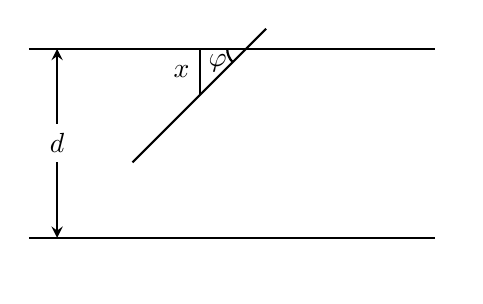
\begin{tikzpicture}[thick,>=stealth,scale=1.2]
            \draw (-0.3,1) -- (4,1) (-0.3,-1)--(4,-1)
            node[below]{\phantom{$O$}};
            \draw[<->] (0,1) -- (0,-1)node[midway,fill=white]{$d$};
            \draw (2,1) -- +(45:0.3) --+ (-135:1.7);
            \draw (1.8,1) arc (180:225:0.2);
            \draw (1.51,1) --node[left]{$x$} ++(0,-0.49);
            \node at (1.7,0.85){$\varphi$};
        \end{tikzpicture}
        \caption{蒲丰投针问题}.
        \label{fig1.2.4}
    \end{minipage}
    \begin{minipage}[b]{0.5\linewidth}
        \centering
        \begin{tikzpicture}[thick,>=stealth]
            \draw[->](-0.3,0) -- (0,0)node[below]{$O$}
            -- (pi,0)node[below]{$\pi$} -- (4.2,0) node[below]{$\varphi$};
            \draw[->](0,0) -- (0,2.2)node[left]{$d/2$}
            -- (0,3) node[right]{$x$};
            \draw (0,2.2)--(pi,2.2)node[above right]{$\Omega$} -- (pi,0);
            \filldraw[pattern=north east lines]
            (0,0)-- plot[domain=0:pi,samples=100](\x,{1.3*sin(\x r)}) -- (pi,0)--cycle;
            \node at (1.57,1.6){$\frac l2\sin\varphi$};
        \end{tikzpicture}
        \caption{蒲丰投针问题中的$\Omega$和$A$}.
        \label{fig1.2.5}
    \end{minipage}
\end{figure}

\begin{example}
    在长度为$a$的线段内任取两点将其分为三段,求它们可以构成一个三角形的概率。
\end{example}

\begin{solution}
    由于是将线段任意分成三段,所以由等可能性知这是一个几何概率问题。分别用$x$,$y$和$a - x - y$表示线段被分成的三段长度,见图\ref{fig1.2.6}。则显然应该有
    \[ 0 < x < a; \quad 0 < y < a; \quad 0 < a - (x + y) < a \]
    第三个式子等价于:$0 < x + y < a$。所以样本空间为(见图\ref{fig1.2.7})
    \[ \Omega = \{(x, y): 0 < x < a, 0 < y < a, 0 < x + y < a\} \]
   $\Omega$的面积为
    \[ S_\Omega = \frac{a^2}{2} \]

    又根据构成三角形的条件:三角形中任意两边之和大于第三边,得事件$A$所含样本点$(x,y)$必须满足:
    \begin{align*}
         & 0 < a - (x + y) < x + y, \\
         & 0 < x < y + (a - x - y), \\
         & 0 < y < x + (a - x - y).
    \end{align*}
    整理得
    \[ \frac{a}{2} < x + y < a;\quad 0 < x < \frac{a}{2}; \quad 0 < y < \frac{a}{2} \]
    所以事件$A$可用图~\ref{fig1.2.8} 中的阴影部分表示。事件$A$的面积为
    \[ S_A = \frac{a^2}{8}. \]
    由此得
    \[P(A) = \frac1{4}. \]
\end{solution}

\begin{figure}
    \begin{minipage}[b]{0.3\linewidth}
        \centering
        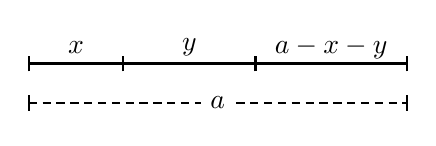
\begin{tikzpicture}[thick,>=stealth,xscale=1.2]
            \draw (0,0) -- (4,0);
            \draw [densely dashed,yshift=-0.5cm](0,0) -- (4,0) node[midway,fill=white]{$a$};
            \foreach \x in {0,1,2.4,4}
            \draw(\x,-0.1) -- (\x,0.1);
            \draw[yshift=-0.5cm](0,-0.1)--(0,0.1)
            (4,-0.1)--(4,0.1);
            \draw (0.5,0.2)node{$x$} (1.7,0.2)node{$y$}
            (3.2,0.2)node{$a-x-y$};
        \end{tikzpicture}
        \caption{长度为$a$的线段分成三段.}
        \label{fig1.2.6}
    \end{minipage}
    \begin{minipage}[b]{0.3\linewidth}
        \centering
        \begin{tikzpicture}[thick,>=stealth,scale=2.6]
            \draw[->] (-0.2,0) --(1,0)node[below]{$a$}-- (1.5,0)node[below]{$x$};
            \draw[->] (0,-0.2) --(0,0)node[below left]{$O$}
            --(0,1)node[left]{$a$} -- (0,1.2)node[left]{$y$};
            \filldraw[pattern=horizontal lines] (0,0)--(1,0)
            --(0,1)--cycle;
        \end{tikzpicture}
        \caption{线段分成三段的样本空间}
        \label{fig1.2.7}
    \end{minipage}
    \begin{minipage}[b]{0.3\linewidth}
        \centering
        \begin{tikzpicture}[thick,>=stealth,scale=2.6]
            \draw[->] (-0.2,0) --(1,0)node[below]{$a$}-- (1.5,0)node[below]{$x$};
            \draw[->] (0,-0.2) --(0,0)node[below left]{$O$}
            --(0,1)node[left]{$a$}--(0,1.2)node[left]{$y$};
            \draw (0,1) -- (1,0);
            \filldraw[pattern=horizontal lines]
            (0.5,0)node[below]{$1/2$} -- (0.5,0.5)
            --(0,0.5)node[left]{$1/2$} -- cycle;
        \end{tikzpicture}
        \caption{构成三角形的条件}
        \label{fig1.2.8}
    \end{minipage}
\end{figure}

\subsection{Bertrand奇论}

在一圆内任取一条弦,问其长度超过该圆内接等边三角形的边长的概率是多少?这是一个几何概率问题,它有三种解法,具体如下:
\begin{enumerate}
    \item 由于对称性,可只考察某指定方向的弦。作一条直径垂直于这个方向。显然,只有交直径于1/4与3/4之间的弦才能超过正三角形的边长(见图),如此,所求概率为 1/2。
    \item 由于对称性,可让弦的一端点固定,让另一端点在圆周上作随机移动。若在固定端点作一切线,则与此切线夹角在60°与120°之间的弦才能超过正三角形的边长(见图),如此,所求概率为1/3。
    \item 圆内弦的位置被其中点唯一确定。在圆内作一同心圆,其半径仅为大圆半径的一半,则大圆内弦的中点落在小圆内,此弦长才能超过正三角形的边长(见图),如此,所求概率为1/4。
\end{enumerate}

同一问题有三种不同答案,究其原因在圆内“取弦”时规定尚不够具体,不同的“等可能性假定”导致了不同的样本空间。具体如下:其中
“均匀分布”应理解为“等可能取点”。
\begin{enumerate}
    \item 解法一中假定弦的中点在直径上均匀分布,直径上的点组成样本空间
    \item 解法二中假定弦的另 一 活动端点在圆周上均匀分布,圆周上的点组成样本空间
    \item 解法三中假定弦的中点在大圆内均匀分布,大圆内的点组成样本空间
\end{enumerate}

可见,上述三个答案是针对三个不同样本空间引起的,它们都是正确的,贝特朗奇论引起人们注意,在定义概率时要事先明确指出样本空间是什么.

\section{条件概率与独立}

\subsection{条件概率}

\begin{definition}[条件概率]
    设$A,B \in \mathscr{F}$,且$P(B)>0$称
    \[ P(A|B) = \frac{P(A \cap B)}{P(B)}\]
    为基于于$B$的\textbf{条件概率}(probability conditional on $B$)。
\end{definition}

\begin{proposition}
    条件概率仍是一个概率测度,即若设$P(B) > 0$,则
    \begin{itemize}
        \item$P(A|B) \ge 0, \quad A \in \mathscr{F}$,
        \item$P(\Omega|B) = 1$,
        \item 若$\mathscr{F}$中的$A_1, A_2, \cdots , A_n, \cdots$互不相容,则
              \[ P \biggl( \bigcup_{n=1}^{+\infty} A_n | B \biggr) = \sum_{n=1}^{+\infty} P(A_n | B) \]
    \end{itemize}
\end{proposition}
\begin{proof}
    从条件概率的定义很容易得出前两点。因为$A_1, A_2, \cdots , A_n, \cdots$互不相容,所以$A_1B, A_2B, \cdots , A_nB, \cdots$也互不相容,故
    \begin{align*}
        P \biggl( \bigcup_{n=1}^{+\infty} A_n | B \biggr)
         & = \frac{P \Biggl( \biggl( \bigcup_{n=1}^{+\infty} A_n \biggr) B \Biggr)}{P(B)}
        = \frac{P \biggl( \bigcup_{n=1}^{+\infty} (A_n B) \biggr)}{P(B)}                  \\
         & = \sum_{n=1}^{+\infty} \frac{P(A_n B)}{P(B)}
        = \sum_{n=1}^{+\infty} P(A_n | B).
    \end{align*}
\end{proof}

\begin{theorem}[乘法法则]
    设$A,B \in \mathscr{F}$,且$P(B)>0$,则
    \[ P(AB) = P(A|B)P(B) \]
    泛化后有:
    \[ P(A_1 A_2 \cdots A_n) = P(A_{1})P(A_2|A_1)P(A_3|A_1 A_2) \cdots P(A_n|A_1 A_2 \cdots A_{n-1}) \]
\end{theorem}

\begin{example}[罐子模型]\label{ex:pot_model}
    设罐中有$b$个黑球、$r$个红球,每次随机取出一个球,取出后将原球放回,还加进$c$个同色球和$d$个异色球。记$B_i$为“第$i$次取出的是黑球”,$R_j$为“第$j$次取出的是红球”。若连续从罐中取出三个球,其中有两个红球、一个黑球。则由乘法公式我们可得
    \begin{align*}
        P(B_1 R_2 R_3)
         & = P(B_1) P(R_2 | B_1) P(R_3 | B_1 R_2)                       \\
         & = \frac{b}{b+r} \frac{r+d}{b+r+c+d} \frac{r+d+c}{b+r+2c+2d}, \\
        P(R_1 B_2 R_3)
         & = P(R_1) P(B_2 | R_1) P(R_3 | R_1 B_2)                       \\
         & = \frac{r}{b+r} \frac{b+d}{b+r+c+d} \frac{r+d+c}{b+r+2c+2d}, \\
        P(R_1 R_2 B_3)
         & = P(R_1) P(R_2 | R_1) P(B_3 | R_1 R_2)                       \\
         & = \frac{r}{b+r} \frac{r+c}{b+r+c+d} \frac{b+2d}{b+r+2c+2d}.
    \end{align*}
    以上概率与黑球在第几次被抽取有关.
\end{example}

罐子模型也称为波利亚(Polya)模型,这个模型可以有各种变化,具体见下:
\begin{enumerate}
    \item 当$c=-1$,$d=0$时,即为\textbf{不返回抽样}。此时前次抽取结果会影响后次抽取结果。但只要抽取的黑球与红球个数确定,则概率不依赖其抽出球的次序,都是一样的。此例中有
          \begin{align*}
              P(B_1 R_2 R_3) & = P(R_1 B_2 R_3) = P(R_1 R_2 B_3)        \\
                             & = \frac{br(r-1)}{(b+r) (b+r-1) (b+r-2)}.
          \end{align*}
    \item 当$c=0$,$d=0$时,即为\textbf{返回抽样}。此时前次抽取结果不会影响后次抽取结果。故上述三个概率相等,且都等于
          \[ P(B_1 R_2 R_3) = P(R_1 B_2 R_3) = P(R_1 R_2 B_3) = \frac{br^2}{(b+r)^3} \]
    \item 当$c>0, d=0$时,称为\textbf{传染病模型}。此时,每次取出球后会增加下一次取到同色球的概率,或换句话说,每次发现一个传染病患者,以后都会增加再传染的概率。与前面两个一样,以上三个概率都相等,且都等于
          \begin{align*}
              P(B_1 R_2 R_3) & = P(R_1 B_2 R_3) = P(R_1 R_2 B_3)       \\
                             & = \frac{br(r+c)}{(b+r)(b+r+c)(b+r+2c)}.
          \end{align*}
          从以上可以看出:在罐子模型中只要$d=0$,则以上三个概率都相等。即只要抽取的黑球与红球个数确定,则概率不依赖其抽出球的次序,都是一样的。但当$d>0$时,就不同了.
    \item 当$c=0, d>0$时,称为\textbf{安全模型}。此模型可解释为:每当事故发生了 (红球被取出),安全工作就抓紧一些,下次再发生事故的概率就会减少;而当事故没有发生时 (黑球被取出),安全工作就放松一些,下次再发生事故的概率就会增大。在这种场合,上述三个概率分别为
          \begin{align*}
               & P(B_1 R_2 R_3) = \frac{b}{b+r} \frac{r+d}{b+r+d} \frac{r+d}{b+r+2d}, \\
               & P(R_1 B_2 R_3) = \frac{r}{b+r} \frac{b+d}{b+r+d} \frac{r+d}{b+r+2d}, \\
               & P(R_1 R_2 B_3) = \frac{r}{b+r} \frac{r}{b+r+d} \frac{b+2d}{b+r+2d}.
          \end{align*}
\end{enumerate}

\begin{theorem}[全概率公式]
    设可列个事件$B_1, B_2, \cdots, B_n, \cdots$互不相容,且包含事件$A$。即$A \subseteq \bigcup_{i=1}^{\infty} B_i,\quad  B_i B_j= \emptyset, \forall i \neq j$,则:
    \[ P(A) = \sum_{i=1}^{\infty} P(B_i) P(A | B_i) ,\quad \forall A \in \mathscr{F}\]
\end{theorem}

\begin{note}
   $P(A | B_i)$可视为事件$A$在$B_i$上的分量,$P(B_i)$则为其权重,加权平均后得到$P(A)$
\end{note}

\begin{proof}
    因为$A \subseteq \bigcup_{i=1}^{\infty} B_i$,所以
    \[ A = A (\bigcup_{n=1}{\infty} B_i) = \bigcup_{i=1}{\infty} (A B_i) \]
    且$AB_1, AB_2, \cdots, AB_n, \cdots$互不相容,所以由可加性得
    \[ P(A) = P \biggl( \bigcup_{i=1}^{\infty} (AB_i) \biggr) = \sum_{i=1}^{\infty} P (AB_i) \]
    再将$P(AB_i) = P(B_i) P(A|B_i)$,代人上式即得全概率公式。
\end{proof}

\begin{corollary}
    \[ P(A) = P(B) P(A|B) + P(\overline{B}) P(A|\overline{B}) \]
\end{corollary}

\begin{example}[敏感性问题调查]
    学生阅读黄色书刊和观看黄色影像会严重影响学生身心健康发展。但这属个人隐私行为。现在要设计一个调查方案,从调查数据中估计出学生中阅读黄色书刊和观看黄色影像的比率$p$.
\end{example}

敏感性问趣的调查方案,关键要使被调查者愿意作出真实回答又能保守个人秘密。经过多年研究和实践,一些心理学家和统计学家设计了一种调查方案,在这个方案中被调查者只需回答以下两个问题中的一个问题,而且只需回答“是”或“否”。
\begin{itemize}
    \item 你的生日是否在7月1日之前?
    \item 你是否看过黄色书刊或影像?
\end{itemize}

这个调查方来看似简单,但为了消除被调查者的顾虑,使被调查者确信他这次调查不会泄露个人秘密,在操作上有以下关键点:
\begin{itemize}
    \item 被调查者在没有旁人的情况下,独自一人回答问题.
    \item 被调查者从只有白球和红球的罐子中随机抽一只球,看过颜色后放回。若抽到白球,则回答问题A;若抽到红球,则回答问题B。
\end{itemize}
如此的调查方法,主要在于旁人无法知道被调查回答的是问题 A 还是问题 B,由此可以极大地消除被调查者的顾虑。现在的问题是如何分析调查的结果。很显然,我们只对问题B是感兴趣。

首先假设有$n$张答卷($n$较大),其中有$k$张回答“是”。有两个信息我们是预先知道的:
\begin{itemize}
    \item 在参加人数较多的情况,任选一人其生日在7月1日之前的概率为0.5.
    \item 罐中红球的比率$\pi$。
\end{itemize}

由全概率公式得
\[ P(\text{是}) = P(\text{白球}) P(\text{是} | \text{白球}) + P(\text{红球}) P(\text{是} | \text{红球}) \]
将$P(\text{红球}) = \pi, P(\text{白球}) = 1-\pi, P(\text{是} | \text{白球}) = 0.5, P(\text{是} | \text{红球}) = p$代入上式右边,而上式左边用频率$k/n$代替概率$P (\text{是})$,得
\[ \frac{k}{n} = 0.5 (1 - \pi) + p \cdot \pi \]
由此得
\[ p = \frac{k/n - 0.5(1 - \pi)}{\pi} \]

\begin{theorem}[Bayes定理]\label{thm:Bayes_Theorem}
    设可列个事件$B_1, B_2, \cdots, B_n, \cdots$互不相容,且包含事件$A$。即$A \subseteq \bigcup_{i=1}^{\infty} B_i,\quad  B_i B_j= \emptyset, \forall i \neq j$,则
    \[ P(B_i | A) = \frac{P(B_i) P(A|B_i)}{\sum_{j=1}^n P(B_j) P(A|B_j)} \]
\end{theorem}

\begin{example}
    某地区居民的肝癌发病率为\num{0.0004},现用甲胎蛋白法进行普查。医学研究表明,化验结果是存有错误的。已知患有肝癌的人其化验结果 \SI{99}{\percent} 呈阳性 (有病),而没患肝癌的人其化验结果 \SI{99.9}{\percent} 呈阴性 (无病)。现某人的检查结果呈阳性,求其真患肝癌的概率。
\end{example}
\begin{solution}
    记$B$为事件“被检查者患有肝癌”,$A$为事件“检查结果呈阳性”。由题设知
    \begin{gather*}
        P(B) = 0.0004, \quad P(\overline{B}) = 0.996,\\
        P(A|B) = 0.99, \quad P(A|\overline{B}) = 0.001.
    \end{gather*}
    由贝叶斯公式得
    \begin{align*}
        P(B|A) & = \frac{P(B) P(A|B)}{P(B) P(A|B) + P(\overline{B}) P(A|\overline{B})} \\
               & = \frac{0.0004 \times 0.99}{0.0004 \times 0.99 + 0.9996 \times 0.001} \\
               & = 0.284.
    \end{align*}
\end{solution}

条件概率的三公式中:乘法公式是求事件交的概率;全概率公式是求一个复杂事件的概率;而贝叶斯公式是求一个条件概率。在贝叶斯公式中,称$P(B_i)$为$B_i$的\textbf{先验概率},称$P(B_i |A)$为$B_i$的\textbf{后验概率}。贝叶斯公式是专门用于计算后验概率的,也就是通过$A$的发生这个新信息,来对$B_i$的概率作出的修正。

\subsection{独立性}

\begin{definition}[事件的独立性]
    如果$A,B\in\mathscr{F}$满足
    \[ P(A\cap B) = P(A)P(B), \]
    则称$A$与$B$\textbf{独立}(independent), 记为$A \indep B$.
\end{definition}
\begin{note}
    当$P(A)>0$时,$P(B|A) = P(B) \iff B \indep A$, 由此可得到\underline{$B$独立于$A$}的直观理解
\end{note}

\begin{property}
    独立性是对称的, 即$A \Vbar B \iff B \Vbar A$. 若两事件独立, 则其补集也独立.
    \begin{center}
        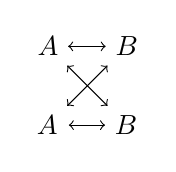
\begin{tikzpicture}
            \node[draw=none,fill=none] (1) at(0,0) {$A^{\complement}$};
            \node[draw=none,fill=none] (2) at(1,0) {$B^{\complement}$};
            \node[draw=none,fill=none] (3) at(0,1) {$A$};
            \node[draw=none,fill=none] (4) at(1,1) {$B$};
            \draw[<->] (1)--(2);
            \draw[<->] (1)--(4);
            \draw[<->] (3)--(2);
            \draw[<->] (3)--(4);
        \end{tikzpicture}
    \end{center}
\end{property}
\begin{proof}
    由概率的性质知
    \[ P(A \overline{B}) = P(A) - P(AB) \]
    又由$A$与$B$的独立性知
    \[ P(AB) = P(A)P(B) \]
    所以
    \[ P(A \overline{B}) = P(A) - P(A)P(B) = P(A) [1 - P(B)] = P(A)P( \overline{B}) \]
    这表明$A$与$\overline{B}$独立. 类似可证$\bar A$与$\overline{B}$独立,$\bar A$与$B$独立.
\end{proof}

\begin{example}
    有两名选手比赛射击,轮流对同一目标进行射击,甲命中目标的概率为$\alpha$,乙命中目标的概率为$\beta$。甲先射,谁先命中谁得胜。问甲、乙两人获胜的概率各为多少?
\end{example}
\begin{solution}
    记事件$A_i$为“第i次射击命中目标”,因为甲先射,所以事件“甲获胜”可以表示为
    \[ A_1 \cup \bar A_1\bar A_2 A_3 \cup \bar A_1\bar A_2\bar A_3\bar A_4A_5\cup\cdots \]
    又因为各次射击是独立的,所以得
    \begin{align*}
        P(\text{甲获胜}) & = \alpha + (1-\alpha)(1-\beta)\alpha + (1-\alpha)^2(1-\beta)^2\alpha + \cdots \\
                      & = \alpha\sum_{i=0}^{+\infty}(1-\alpha)^i(1-\beta)^i                           \\
                      & = \frac{\alpha}{1-(1-\alpha)(1-\beta)}.
    \end{align*}
    同理可得
    \begin{align*}
        P(\text{乙获胜}) & = P(\bar A_1A_2\cup \bar A_1\bar A_2\bar A_3A_4\cup\cdot)       \\
                      & = (1-\alpha)\beta + (1-\alpha)(1-\beta)(1-\alpha)\beta + \cdots \\
                      & \beta (1-\alpha)\sum_{i=0}^{+\infty}(1-\alpha)^i(1-\beta)^i     \\
                      & = \frac{\beta(1-\alpha)}{1-(1-\alpha)(1-\beta)}.
    \end{align*}
\end{solution}

\begin{example}
    系统由多个元件组成,且所有元件都独立地工作.设每个元件正常工作的概率都为$p=0.9$,试求以下系统正常工作的概率.
    \begin{enumerate}
        \item 串联系统$S_1$: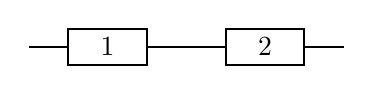
\begin{tikzpicture}[baseline=(a.base),thick]
                  \draw (0,0) -- (4,0);
                  \node(a)[minimum width=1cm,minimum height=0.4cm,draw,fill=white] at (1,0){1};
                  \node[minimum width=1cm,minimum height=0.4cm,draw,fill=white] at (3,0){2};
              \end{tikzpicture}
        \item 并联系统$S_2$: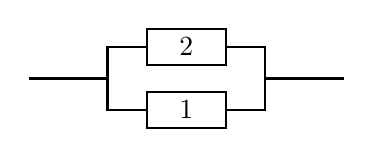
\begin{tikzpicture}[baseline=(a.base),thick,
                      every node/.style =
                          { minimum width=1cm,minimum height=0.4cm,draw,fill=white}]
                  \node[draw = white](a) at (2,0) {};
                  \draw (0,0) -- (1,0)  (3,0) -- (4,0)
                  (1.5,-0.4) -- (1,-0.4) -- (1,0.4) -- (1.5,0.4)
                  (2.5,-0.4) -- (3,-0.4) -- (3,0.4) -- (2.5,0.4);
                  \node at (2,-0.4) {1} ;
                  \node at (2,0.4) {2} ;
              \end{tikzpicture}
        \item 5个元件组成的桥式系统$S_3$: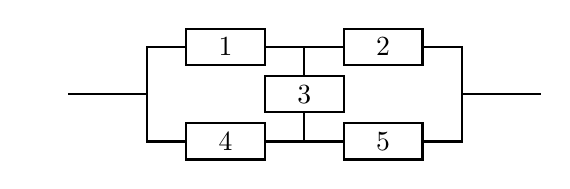
\begin{tikzpicture}[baseline=(a.base),thick,
                      every node/.style =
                          { minimum width=1cm,minimum height=0.4cm,draw,fill=white}]
                  \node[draw = white] (a) at (0,0) {};
                  \draw (0,0) -- (1,0) (3,-0.6) -- (3,0.6) (5,0) -- (6,0)
                  (1,0.6) -- (1,-0.6) -- (5,-0.6) -- (5,0.6) -- cycle;
                  \node at (2,-0.6) {4};
                  \node at (2,0.6) {1};
                  \node at (3,0) {3};
                  \node at (4,0.6) {2};
                  \node at (4,-0.6) {5};
              \end{tikzpicture}
    \end{enumerate}
\end{example}

\begin{solution}
    设$S_i=$“第$i$个系统正常工作”,$A_i=$“第$i$个元件正常工作”.
    \begin{itemize}[(1)]
        \item 对申联系统而言,“系统正常工作”相当于“所有元件正常工作”,即$S_1=A_1A_2$,所以
              \[ P(S_1) = P(A_1A_2) = P(A_1)P(A_2) = p^2 = 0.81 \]
        \item 对并联系统而言,“系统正常工作”相当于“至少一个元件正常工作”,即$S_2=A_1\cup A_2$,所以
              \[ P(S_2) = P(A_1\cup A_2) = P(A_1) + P(A_2) - P(A_1A_2)= p + p - p^2 = 0.99 \]
              或
              \begin{align*}
                  P(S_2) & = 1 - P(\bar S_2) = 1 - P(\bar{A_1\cup A_2}) = 1 - P(\bar A_1\cap \bar A_2) \\
                         & = 1 - P(\bar A_1)P(\bar A_2) = 1 - (1-p)^2 = 0.99.
              \end{align*}
        \item 在桥式系统中,第3个元件是关键,我们先用全概率公式得
              \[ P(S_3) = P(A_3)P(S_3|A_3) + P(\bar A_3)P(S_3|\bar A_3) \]
              因为在“第3个元件正常工作”的条件下,系统成为先并后串系统(见图 \ref{fig1.5.1})。所以
              \begin{align*}
                  P(S_3|A_3) & = P\big( ( A_1\cup A_4 )(A_2 \cup A_5) \big) = P(A_1\cup A_4)P(A_2\cup A_5) \\
                             & = [ 1 - (1-p)^2 ]^2 = 0.9801.
              \end{align*}
              又因为在“第3个元件不正常工作”的条件下,系统成为先串后并系统(见图 \ref{fig1.5.2}).
    \end{itemize}
    \begin{figure}[!ht]
        \centering
        \begin{minipage}{0.48\linewidth}
            \centering
            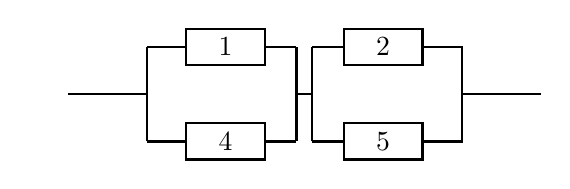
\begin{tikzpicture}[baseline=(a.base),thick,
                    every node/.style =
                        { minimum width=1cm,minimum height=0.4cm,draw,fill=white}]
                \node[draw = white] (a) at (0,0) {};
                \draw (0,0) -- (1,0) (2.9,0) -- (3.1,0)
                (5,0) -- (6,0) (2.9,-0.6) -- (2.9,0.6)
                (3.1,-0.6) -- (3.1,0.6)
                (1,0.6) -- (1,-0.6)(2.9,-0.6) (3.1,-0.6)-- (5,-0.6) -- (5,0.6) -- (3.1,0.6) (2.9,0.6) -- cycle;
                \draw (1,0.6) -- (2.9,0.6) (1,-0.6) -- (2.9,-0.6);
                \node at (2,-0.6) {4};
                \node at (2,0.6) {1};
                \node at (4,0.6) {2};
                \node at (4,-0.6) {5};
            \end{tikzpicture}
            \caption{先并后串系统\label{fig1.5.1}}
        \end{minipage}
        \begin{minipage}{0.48\linewidth}
            \centering
            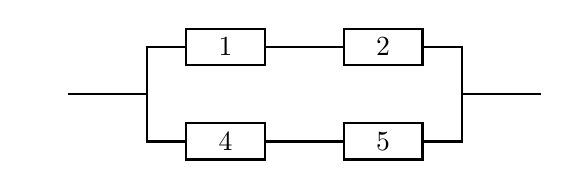
\begin{tikzpicture}[baseline=(a.base),thick,
                    every node/.style =
                        { minimum width=1cm,minimum height=0.4cm,draw,fill=white}]
                \node[draw = white] (a) at (0,0) {};
                \draw (0,0) -- (1,0)  (5,0) -- (6,0)
                (1,0.6) -- (1,-0.6) -- (5,-0.6) -- (5,0.6) -- cycle;
                \node at (2,-0.6) {4};
                \node at (2,0.6) {1};
                \node at (4,0.6) {2};
                \node at (4,-0.6) {5};
            \end{tikzpicture}
            \caption{先串后并系统\label{fig1.5.2}}
        \end{minipage}
    \end{figure}
    所以
    \[ P(S_3|\bar A_3) = P(A_1A_2|\cup A_4A_5) = 1 - (1-p^2)^2 = 0.9639 \]
    最后得
    \begin{align*}
        P(S_3) & = p [ 1-(1-p)^2 ]^2 + (1-p)[ 1-(1-p^2)^2 ]       \\
               & = 0.9\times 0.9801 + 0.1 \times 0.9639 = 0.9785.
    \end{align*}
\end{solution}

\begin{definition}[相互独立]
    对于事件集$A_1, A_2, \dotsc, A_n$, 若对于其中任意子集$A_{i_1}, A_{i_2}, \dotsc, A_{i_n}$有:
    \[ P(A_{i_1} \cap \cdots  \cap A_{i_n}) =P(A_{i_1})\cdots P(A_{i_n})  \]
    则称此事件集\textbf{相互独立}(mutually independent)
\end{definition}
\begin{remark}
    各事件两两独立不能推出所有事件相互独立。
\end{remark}

\begin{example}[伯恩斯坦反例]
    一个均匀的正四面体,其第一面染成红色,第二面染成白色,第三面染成黑色,而第四面同时染上红,白,黑三种颜色.现在以$A,B,C$分别记投一次四面体出现红,白,黑颜色朝下的事件,则由于在四面体中有两面有红色,因此$P(A)=\frac{1}{2}$。同理$P(B)=P(C)=\frac{1}{2}$,同时易得$P(AB) = P(BC)= P(AC) =\frac{1}{4}$。所以$A,B,C$两两独立,但是$P(ABC)=\frac{1}{4}\neq P(A)P(B)P(C)$,从而$A,B,C$不相互独立。
\end{example}

\begin{definition}[事件域的独立性]
    若$\mathscr{G} \subset \mathscr{F}$与$\mathscr{H} \subset \mathscr{F}$满足
    \[ A \Vbar B, \quad \forall A\in\mathscr{G},\ B\in\mathscr{H}, \]
    则称$\mathscr{G}$与$\mathscr{H}$独立, 记为$\mathscr{G} \Vbar \mathscr{H}$
\end{definition}

测度论告诉我们一个重要结果: 如果$\mathscr{G}$对交集运算封闭, 那么成立$\mathscr{G}\Vbar\mathscr{H} \implies \sigma(\mathscr{G}) \Vbar \mathscr{H}$,其中$\sigma(\mathscr{G})$是$\mathscr{G}$扩张而成的一个合适的最小的$\sigma$代数, 定义为所有包含$\mathscr{G}$的$\sigma$代数的交集。

类似地可以定义$n$个试验$E_1,E_2,\cdots,E_n$的相互独立性:如果$E_1$的任一结果、$E_2$的任一结果$\cdots\cdots E_n$的任一结果都是相互独立的事件,则称\textbf{试验$E_1,E_2,\cdots,E_n$相互独立}。

\begin{definition}[Bernouli试验]\label{def:Bernouli_experiment}
    如果$n$个独立试验是相同的,则称其为$n$重\textbf{独立重复试验}。如果在$n$重独立重复试验中,每次试验的可能结果为两个:$A$或$\bar A$,且每次实验事件$A$发生的概率不变,则称这种试验为$n$重\textbf{Bernouli试验}。
\end{definition}

\begin{problemset}[错题记录]
    \item (茆1.2.4)从一副52张的扑克牌中任取4张,求下列事件的概率:
    \begin{enumerate}
        \item 全是黑桃;
        \item 同花;
        \item 没有两张同一花色;
        \item 同色.
    \end{enumerate}
    \item (茆1.2.5)考虑一元二次方程$x^2+Bx+C=O$,其中$B,C$分别是将一颗骰子接连掷两次先后出现的点数,求该方程有实根的概率和有重根的概率
    \item (茆1.2.10)从$n$个数$1, 2, \cdots, n$中任取2个,问其中一个小于$k (1 < k < n)$,另一个大于$k$的概率是多少?
    \item (茆1.2.13)把10本书任意地放在书架上,求其中指定的三本书放在一起的概率.
    \item (茆1.2.19)$n$个男孩,$m$个女孩($m \le n + 1$)随机地排成一排,试求任意两个女孩都不相邻的概率.
    \item (茆1.2.20)将3个球随机地放入4个杯子中去,求杯子中球的最大个数分别为1, 2, 3的概率各为多少?
    \item (茆1.2.22)将$n$个完全相同的球 (这时也称球是不可辨的) 随机地放入$N$个盒子中,试求恰好有$m$个空盒的概率
    \item (茆1.2.23)在区间$(0,1)$中随机地取两个数,求事件“两数之和小于7/5”的概率.
    \item (茆1.3.4)从$0, 1, 2, \cdots ,9$十个数字中任意选出三个不同的数字,试求事件“三个数字中含 0 但不含 5”的概率
    \item (茆1.3.8)从数字$1, 2, \cdots ,9$中可重复地任取$n$次,求$n$次所取数字的乘积能被$10$整除的概率.
    \item (茆1.3.23)证明:$\lvert P(AB) - P(A)P(B) \rvert \le \frac1{4}$
    \item (茆1.4.6)$n$件产品中有$m$件不合格品,从中任取两件,已知两件中有一件是合格品,求另 一件也是合格品的概率
    \item (茆1.4.27)口袋中有$a$个白球,$b$个黑球和$n$个红球,现从中一个一个不返回地取球.试证白球比黑球出现得早的概率为$\frac{a}{a+b}$,与$n$无关.
    \item (茆1.5.20)甲、乙、丙三人进行比赛,规定每局两个人比赛,胜者与第三人比赛,依次循环,直至有一人连胜两次为止,此人即为冠军.而每次比赛双方取胜的概率都是1/2,现假定甲、乙两人先比,试求各人得冠军的概率.
    \item (茆1.5.21)甲、乙两个赌徒在每一局获胜的概率都是1/2.两人约定谁先赢得一定的局数就获得全部赌本.但赌博在中途被打断了,请问在以下各种情况下,应如何合理分配赌本:
    \begin{enumerate}
        \item 甲、乙两个赌徒都各需赢$k$局才能获胜;
        \item 甲赌徒还需赢2局才能获胜,乙赌徒还需赢3局才能获胜;
        \item 甲赌徒还需赢$n$局才能获胜,乙赌徒还需赢$m$局才能获胜.
    \end{enumerate}
    \item (李1.23)任意从数列$1,2,\cdots,N$中有放回地取出$n$个数并按大小排列成:$x_1\le x_2\le \cdots \le x_n$,试求$x_m=M$的概率。
    \item (李1.38)(赠券收集)食品厂把印有水浒108 将之一的画卡作为赠券装人某种儿童食品袋中,每袋一卡,试求购买$n$袋这种食品而能收齐全套画卡的概率。
    \item (李1.40)有$w$个白球与$b$个黑球任你放人两个袋子中,让你的朋友随机抽一袋并从中摸出一只球,你将如何做以使你的朋友摸得黑球的概率最大。
    \item (李1.42)父,母,子三人举行比赛,每局总有一人胜一人负(没有和局),每局的优胜者就与未参加此局的人再进行比赛,如果某人首先胜了两局,则他就是整个比赛的优胜者,由父决定第一局由哪两人参加,其中儿子实力最强,所以父为了使自己得胜的概率达到最大,就决定第一局由他与妻子先比赛,试证父的决策为最优策略(任何一对选手中一人胜对方的概率在整个比赛中是不变的).
\end{problemset}
